\newcommand{\CLASSINPUTbaselinestretch}{1.0} % baselinestretch
\newcommand{\CLASSINPUTinnersidemargin}{1in} % inner side margin
\newcommand{\CLASSINPUToutersidemargin}{0.5in} % outer side margin
\newcommand{\CLASSINPUTtoptextmargin}{0.5in}   % top text margin
\newcommand{\CLASSINPUTbottomtextmargin}{0.5in}% bottom text margin

\documentclass{llncs}

\usepackage[nocompress]{cite}
\usepackage{indentfirst}
\usepackage{graphicx}
% http://www.ctan.org/pkg/graphicx
% http://www.tug.org/applications/pdftex

\usepackage{algorithm}
% http://www.ctan.org/pkg/algorithms

\usepackage{array}
% http://www.ctan.org/pkg/array

\usepackage{mdwtab}
\usepackage{eqparbox}
\usepackage[caption=false,font=footnotesize,labelfont=sf,textfont=sf]{subfig}
% http://www.ctan.org/pkg/subfig

\usepackage{algpseudocode}
\usepackage{pifont}

% correct bad hyphenation here
\hyphenation{op-tical net-works semi-conduc-tor}

\begin{document}

\title{Automatic Vehicle Accident Report\\ and Analysis}

\author{N.Md~Faizaan, 2013103512\\
        G.Aravind, 2013103004\\
        Gaurav~Agarwal, 2013103505}%

\authorrunning{Faizaan, Arvind, Gaurav}
\institute{College of Engineering, Guindy}
\maketitle

\begin{abstract}
Road transportation has revolutionized the way we travel and transport goods. The increasing number of road users is proportionate with the increasing number of accidents, which could include fatalities. Reporting accidents has its challenges; mainly there exist communication gap in relaying location information to the operator. This, in turn, causes slow response to the situation. The objective of this project is to develop an integrative system that is able to speed up the process of reporting accidents. Our work includes a microcontroller-based low-cost Accident Reporting Unit (ARU) that contains a GPS positioning system and a GSM shield to sense and generate accidental events to a centralized server. Apart from that, it also collects the data and derives conclusions from it.
\keywords{Networking, Embedded, GPS, GSM}
\end{abstract}

\section{Introduction}
\label{sec:introduction}
Road accidents constitute the major part of the accident deaths all over the world. According to the Insurance Institute for Highway Safety (IIHS), new cars and its high-tech safety features have helped to lessen auto related deaths over the past 12 years. Though it credits technology for lessening auto accidents, yet the IIHS cannot help accusing bad driving behavior like drunken driving, speeding and not using seatbelts for still causing major traffic deaths. Automatic vehicle accident detection and report system is an embedded intelligence implanted into the auto- mobile. This project proposes a distributed system which alerts on the occurrence of an accident.

The purpose of the project is to find the vehicle where it is and locate the vehicle by means of sending a message using a system which is placed inside the vehicle. To help the injured first we need to know where the accident happened through location tracking and sending a message to your related one or to the emergency services. Here we use GPS and GSM modules which help to trace the vehicle. The exact location of the vehicle is sent to our remote server using the GSM shield. The assumption is that the micro controller unit (MCU) along with the GPS module is annexed onto to the air bag electronic control unit which is used as a trigger signal to detect the collision. Upon impact, the MCU notifies the emergency services about the accident and also stores this data onto the remote server along with the coordinates obtained from the GPS module, creating a digital record of the incident tagged along with date, time and location. These records could aid the government to flag accident-prone zones thereby assisting them in taking effective precautionary measures. 

\section{Related Works}
There are new automatic accident reporting techniques. These systems are majorly aimed for four wheeler vehicles. Many systems have been proposed for accident detection by researchers. The accident detection methods were first based on real time traffic analysis to forecast traffic flow which deals with the change in the traffic before the occurrence of the accident. This detection technique is known as Traffic-incident detection-algorithm based on nonparametric regression which was proposed by Shuming Tang and Haijiun Gao.

In \cite{chuan}, they instead make use of an smartphone application which is used by the user to report the accident itself. When the driver initiates the report, CCTV is used to confirm the accident before services are called in. This method has its downsides as it has an increased risk of false alarms and delay in detecting an accident through CCTV.

A system proposed in \cite{bin} put forward a design for accident detection and alert system for motor cycles considering three parameters: acceleration/deceleration, tilt of the vehicle and the pressure change on the body of the vehicle. This systems lacks because two wheelers accidents may have a number of scenarios which are not completely covered by this system.

\section{Proposed Works}

Our project describes about the accident report generation using GPS and GSM. We use a micro-controller to detect the accident based on feed from the Airbag deployment unit. The GPS receives the location of the vehicle which is sent to a remote server. The GPS data is used to communicate with the emergency services. We also design an smartphone application which can be used by the user to report false alarms. This is different than most works, which propose that the smartphone itself be used for accident report. 

\section{Architecture}

%TODO - Insert BLOCK diagram here

\subsection{Global Positioning System}

The GPS module handles collection of the geolocational data and passes this data to the MCU. This module is activated by an interrupt from the MCU which is generated whenever an accident is detected by the MCU. The coordinates are formatted into the Payload format (Refer section \ref{sub:payload}) \\


\begin{figure}[h!]
\centering
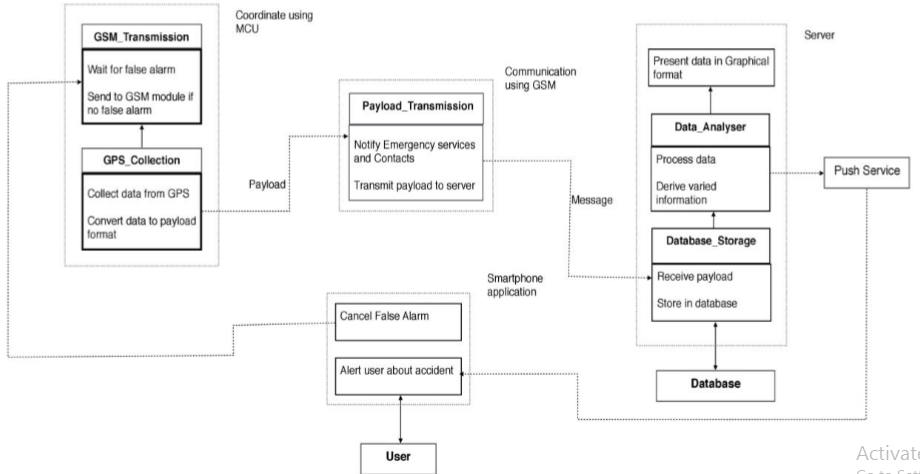
\includegraphics[scale=0.5]{block}
\caption{Block diagram}
\label{fig:block}
\end{figure}


\noindent A pseudocode working of the GPS \\

\begin{verbatim}
On Interrupt
begin
     Collect coordinates
     Format coordinates
end interrupt handler
\end{verbatim}

The GPS might not be accurate in closed locations, but on roads, the data provided by GPS will be of high accuracy.

\subsection{Global System for Mobile Communication}

GSM is a digital mobile telephone system that is widely used in Europe and other parts of the world. The GSM module performs two crucial functions. It receives the payload from the MCU, notifies the emergency services and also transmits the payload to the centralized server.

\begin{verbatim}
if (Payload received)
begin
    Notify Emergency Services
    Send Payload
endif
\end{verbatim}

A small snippet outlining the primary workings of the GSM module.

\noindent\textbf{Notify Emergency Services} \\
\noindent\textbf{Input} : Payload \newline
\textbf{Output} : Result (Success, Error)

\begin{verbatim}
begin
     Get emergency contacts from owner file
     Send payload to the emergency contacts using AT commands
end 
\end{verbatim} 

The ARU contains an owner file which is created when a new user registers. This file contains info about user that is made part of the payload. This payload (\ref{sub:payload}) is sent to the emergency services with the help of AT commands. \\

\noindent\textbf{Send Payload} \\
\noindent\textbf{Input}: AccidentPayload \newline
\textbf{Output} : Log report

\begin{verbatim}
begin
     Send POST request to the server to report new accident
     Include the accidentPayload (in JSON) in the POST request
     Log report if response code is 201
end 
\end{verbatim}

The server accepts a POST request which contains the accident payload. On successful request, it sends a 201 (Content created) response or else returns a 400 (Bad request) upon which, the device schedules a send later. 

\subsection{Arduino Microcontroller}

An Arduino board is the main module of the system. It detects the accident with the help of the Airbag deployment unit and uses the GPS and GSM modules to do the required work.

\begin{verbatim}
Init GPS module
Init GSM module
while (MCU is running)
    Ping Deployment Unit for Accident SIG
    if (SIG == true)
    begin
       Ping GPS module for coordinates
       Convert to payload format
       Send to GSM
    endif
end while
\end{verbatim}

This code snippet initialises and sets up the Microcontroller unit to respond to accidents. Whenever an accident happens, the MCU gets the coordinates from the GPS module, converts into a format recognised by the server and forwards it to the GSM module.

\subsection{Smartphone application}

We make use of a smart-phone application in case of a false alarm. We can't always rely on air bag deployment as an indicator of some serious accidents. There are instances in which air bags are deployed even for some minor accidents and it is not necessary to notify the emergency services. In those cases, the app provides an option to cancel the alarm (i.e. false alarm). The airbag deployment unit triggers the micro-controller unit as well as activates the mobile application. The mobile app allows the user to interrupt further process in case of a false alarm with a timeout of 2 minutes. The GSM module holds the data during that time out. If the alarm has not been cancelled in that particular timeout then the triggered alarm is considered to be genuine and the process continues. The GSM after the timeout notifies the emergency services and sends the data to web server for analysis.

\newpage
\subsection{Activity Diagram}
\begin{figure}[h!]
\centering
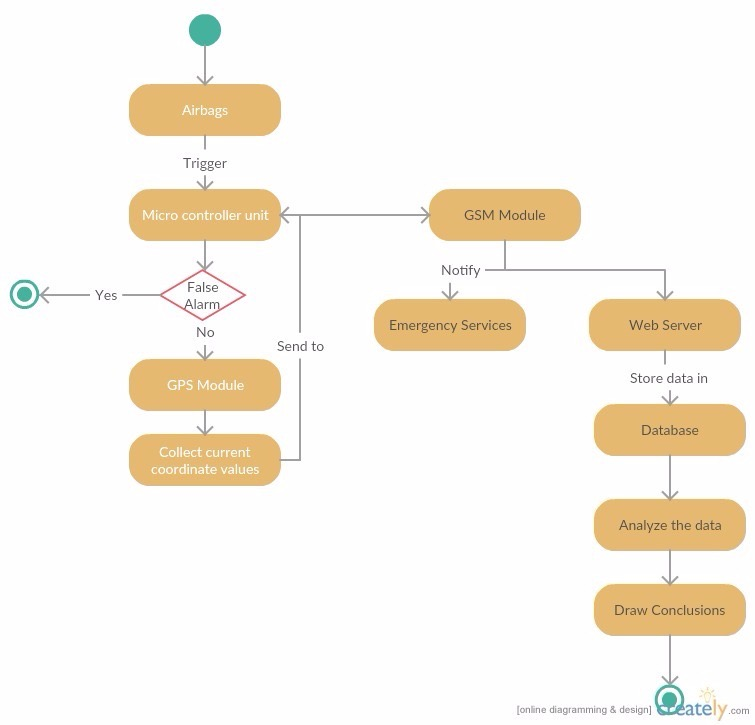
\includegraphics[scale=0.5]{acti}
\caption{Activity diagram}
\label{fig:acti}
\end{figure}

\newpage

\section{Data analysis}
The data stored at the remote server are subjected to analysis with the goal of discovering useful information, suggesting conclusion and supporting decision making. There are different ways of analysing data. These ways are briefly described here.

\subsection{Time series}
A single variable is captured over a period of time, such as the unemployment rate over a 10-year period. A line chart may be used to demonstrate the trend. This is shown in Figure \ref{fig:time}

\begin{figure}[h!]
\centering
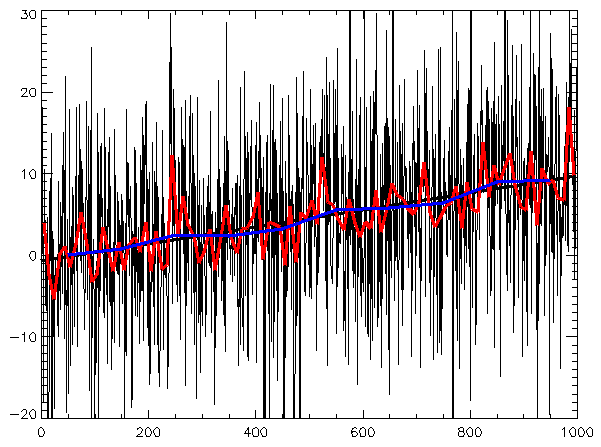
\includegraphics[scale=0.3]{time}
\caption{Time series}
\label{fig:time}
\end{figure}

\subsection{Correlation}
Comparison between observations represented by two variables (X,Y) to determine if they tend to move in the same or opposite directions. For example, plotting unemployment (X) and inflation (Y) for a sample of months. A scatter plot as shown in Figure \ref{fig:scatter} is typically used for this message.

\begin{figure}[h!]
\centering
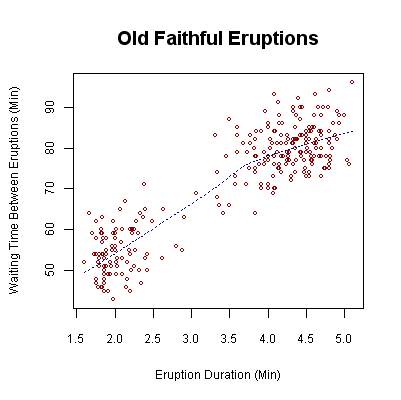
\includegraphics[scale=0.4]{scatter}
\caption{Scatter plot}
\label{fig:scatter}
\end{figure}

\newpage
\subsection{Analytical Activities of the Data Users}
Users may have particular data points of interest within a data set, such low-level user analytic activities are given below

\begin{center}
\begin{tabular}{| m{5em} | m{10em}| m{10em} | m{10em} |} 
\hline
\textbf{Task} & \textbf{General description} & \textbf{Abstract} & \textbf{Examples} \\ 
\hline
Retrieve value & Find attributes from a set & Whta are values of attributes in data cases & Name of victim\\ 
\hline
Compute derived values & Compute an aggregate numeric representation & What is value of aggregate function F over a set S of cases? & What is the average number of accidents ? \\ 
\hline
Find extremum & Find extreme values in data cases & What are the top/bottom data w.r.t attribute A? & Type of vehicles involved in frequent accidents \\
\hline
Sort & Given a set of data cases, rank them according to some ordinal metric & What is the sorted order of a set S of data cases according to value of attribute A? & Order accident based on time \\
\hline
\end{tabular}
\end{center}

\section {Pseudocode}
\subsection{Server}

The server is used to save accident data

\noindent\textbf{Input} : Request \newline
\textbf{Output} : Response

\begin{verbatim}
On GET Request
begin
     Verify AUTH
     if(endpoint == '/db')
          Query DB for all users data
     else if(endpoint == '/db/find')
          Query DB for single user
     else if(endpoint == '/accident/all')
          Query DB for all accident data
     else if(endpoint == '/accident/uuid')
          Query DB for a user’s accident data
     else
          Set status as 404
     endif
     
     Send response
end
\end{verbatim}

This defines all the functions for the different GET requests occur

\begin{verbatim}
On POST request
begin
    Verify AUTH
    if(endpoint == '/db/new')
    begin
        Verify Payload
        Insert into DB
	endif
	if(endpoint == '/accident/new')
	begin
		Verify Form data
		Insert into DB
   endif
   Send response as 201 if INSERT is success else send 400
end	
\end{verbatim}

This defines all the functions for the different POST requests occur.

\begin{verbatim}
On DELETE request
begin
     Verify AUTH
     if(endpoint == ‘/db/remove’)
     begin
          Verify UUID
          Delete from DB
     endif
end
\end{verbatim}

This defines all the functions that occur when DELETE request occurs.

\subsection{Payload Format}
\label{sub:payload}
\begin{verbatim}
{
    UUID: Alphanumeric
    latX: Real
    latY: Real
}
\end{verbatim}

\section{Extensions}
\begin{itemize}
	\item  Used in automotives and transport vehicles- from lighter vehicles like cars, to heavier automotives like ships and aeroplanes
	\item Security and remote monitoring of vehicles especially during military operations. 
	\item This system can also can be interfaced with Vehicle airbag system such that when the sensors detect the accident, the air bags get opened
	\item  This system can also be used for real time monitoring of traffic
\end{itemize}

\section{Conclusion}

A working model of Automatic vehicle accident detection and messaging system using a GPS and GSM modems has been implemented successfully. The biggest advantage of our project is, whenever the sensor is activated we will be immediately getting the acknowledgement from GSM modem to our mobile number. This system locates the accident spot accurately, realizing the automation of accident detection and messaging system. Consequently, it will save the precious time required to save the accident victims. Further this system can be implemented using the vibration sensors as well as the sound sensors, in order to make it more accurate and efficient to detect an accident

\begin{thebibliography}{1}

\bibitem{hanbo}
Wang Wei, Fan Hanbo― \emph{Traffic Accident Automatic Detection And Remote Alarm Device}

\bibitem{taylor}
M. A. P. Taylor – \emph{Intelligent Transport Systems} \\
A handbook of transport systems and traffic control

\bibitem{zhao}
Y. Zhao – \emph{Mobile phone location determination and its impact on intelligent transportation systems}

\bibitem{ching}
Zhing - \emph{Automatic traffic accident detection and alarm system} \\
International Journal of Technological Exploration and Learning 

\bibitem{chuan}
Chuan-zhi, Ru-fu, Hong-wu - \emph{Method of freeway incident detection using wireless positioning} \\
International Conference on Automation and Logistics, Qingdao, China

\bibitem{syed} 
Syedul Amin et al - \emph{Kalman filterted GPS accelerometer-based accident detection and location system: a low-cost approach} \\
Current science

\bibitem{bin}
Basheer et al - \emph{Design of accident detection and alert system for motor cycles} \\ 
Global Humanitarian Technology Conference

\end{thebibliography}

%\vfill

%\enlargethispage{-5in}

\end{document}